\documentclass{article}

\usepackage{amsmath}
\usepackage{amssymb}
\usepackage{hyperref}
\usepackage{indentfirst}
\usepackage{matlab-prettifier}
\usepackage[shortlabels]{enumitem}
\usepackage{graphicx}

%User defined commands
\newcommand{\inv}[1]{#1^{-1}}
\newcommand{\abs}[1]{|#1|}
\newcommand{\norm}[1]{||#1||}
\newcommand{\cond}{\kappa_{||\cdot||}}

\begin{document}
\begin{center}
	\huge{\bf Math 170A: Homework 4} \\
	Merrick Qiu
\end{center}

\section*{Question 1}
\[
    q_1 = \frac{w_1}{2} = \begin{bmatrix} 
        \frac{1}{2} \\ \frac{1}{2} \\ \frac{1}{2} \\ \frac{1}{2} \\
    \end{bmatrix}
\]
\[
    \tilde{q}_2 = \begin{bmatrix} 
        3 \\ 3 \\ -1 \\ -1 \\
    \end{bmatrix} -
    2\cdot \begin{bmatrix} 
        \frac{1}{2} \\ \frac{1}{2} \\ \frac{1}{2} \\\frac{1}{2} \\
    \end{bmatrix}
    = \begin{bmatrix}
        2 \\ 2 \\ -2 \\ -2 \\
    \end{bmatrix}
\]
\[
    q_2 = \frac{\tilde{q}_2}{4} = \begin{bmatrix} 
        \frac{1}{2} \\ \frac{1}{2} \\ -\frac{1}{2} \\ -\frac{1}{2} \\
    \end{bmatrix}
\]
\[
    \tilde{q}_3 = \begin{bmatrix}
        6 \\ 0 \\ 2 \\ 0
    \end{bmatrix}
    - 4 \cdot \begin{bmatrix} 
        \frac{1}{2} \\ \frac{1}{2} \\ \frac{1}{2} \\ \frac{1}{2} \\
    \end{bmatrix}
    - 2 \cdot \begin{bmatrix} 
        \frac{1}{2} \\ \frac{1}{2} \\ -\frac{1}{2} \\ -\frac{1}{2} \\
    \end{bmatrix} = \begin{bmatrix}
        3 \\ -3 \\ 1 \\ -1
    \end{bmatrix}
\]
\[
    q_3 = \frac{\tilde{q}_3}{\sqrt{20}} = \begin{bmatrix}
        \frac{3}{\sqrt{20}} \\ -\frac{3}{20} \\ \frac{1}{20} \\ -\frac{1}{20}
    \end{bmatrix}
\]
\newpage 

\section*{Question 2}
One can take $q_1$ and $q_2$ and append two more vectors that are orthonormal
to them to get a Full QR decomposition of $A$
\[
    A = 
    \begin{bmatrix}
        \frac{1}{2} &  \frac{1}{2} & -\frac{1}{2} & -\frac{1}{2}\\
        \frac{1}{2} &  \frac{1}{2} &  \frac{1}{2} & \frac{1}{2}\\
        \frac{1}{2} & -\frac{1}{2} & -\frac{1}{2} & \frac{1}{2}\\
        \frac{1}{2} & -\frac{1}{2} &  \frac{1}{2} & -\frac{1}{2}\\ 
    \end{bmatrix}
    \begin{bmatrix}
        2 & 2 & 0 \\
        0 & 4 & 0 \\
        0 & 0 & 0 \\
        0 & 0 & 0
    \end{bmatrix}
\]
The minimizer is 
\[
    x= \inv{R}Q^Tb
    = \begin{bmatrix}
        \frac{1}{2} & - \frac{1}{4} & 0 & 0\\
        0 & \frac{1}{4}  & 0 & 0
    \end{bmatrix}
    \begin{bmatrix}
        \frac{1}{2} &  \frac{1}{2} & \frac{1}{2} & \frac{1}{2}\\
        \frac{1}{2} &  \frac{1}{2} &  -\frac{1}{2} & -\frac{1}{2}\\
        -\frac{1}{2} & \frac{1}{2} & -\frac{1}{2} & \frac{1}{2}\\
        -\frac{1}{2} & \frac{1}{2} &  \frac{1}{2} & -\frac{1}{2}\\ 
    \end{bmatrix}
    \begin{bmatrix}
        1 \\ 1 \\ 0 \\ 1
    \end{bmatrix}
    = \begin{bmatrix}
        \frac{5}{8} \\ \frac{1}{8}
    \end{bmatrix}
\]
\newpage 

\section*{Question 3}
\begin{enumerate}
    \item Since for an orthogonal matrix, $\norm{Qx}_2 = \norm{x}_2$ for all $x$,
    we have that $\norm{Q}_2 = 1$, $\norm{\inv{Q}}_2 = 1$, and $\kappa(Q) = 1$.
    \item We can rearrange the equation as 
    \[
        Q\hat{x} = b - \delta Q\hat{x}
    \]
    which is equvalent to perturbing $b$ with 
    $\delta b = -\delta Q \hat{x}$.
    Thus we can say that 
    \[
        \frac{\norm{\delta x}_2}{\norm{\hat{x}}_2} \leq \frac{\norm{\delta Q \hat{x}}_2}{\norm{b}_2}
    \]
\end{enumerate}
\newpage 

\section*{Question 4}
We can write
\[
    A = M^TM = (QR)^TQR = R^T(Q^TQ)R = R^T R
\]
We see that $M$ is a $n \times m$ full rank matrix
and that $R$ is a $m \times m$ upper triangular matrix
that happens to be the Cholesky decomposition of $A$ since 
$R$ times its transpose equals to $A$, which is positive definite.
\newpage 

\section*{Question 5}
We can see that the orthogonal matrix $Q$ differs signficantly
between the two methods but the matrix $R$ is mostly the same
between the two matricies.

orthoQ1 demonstrates that $Q_1$ from classical Gram-Schmidt is very far from being orthogonal,
but orthoQ1 demonstrates that $Q_2$ from modified Gram-Schmidth is much closer to being orthogonal.

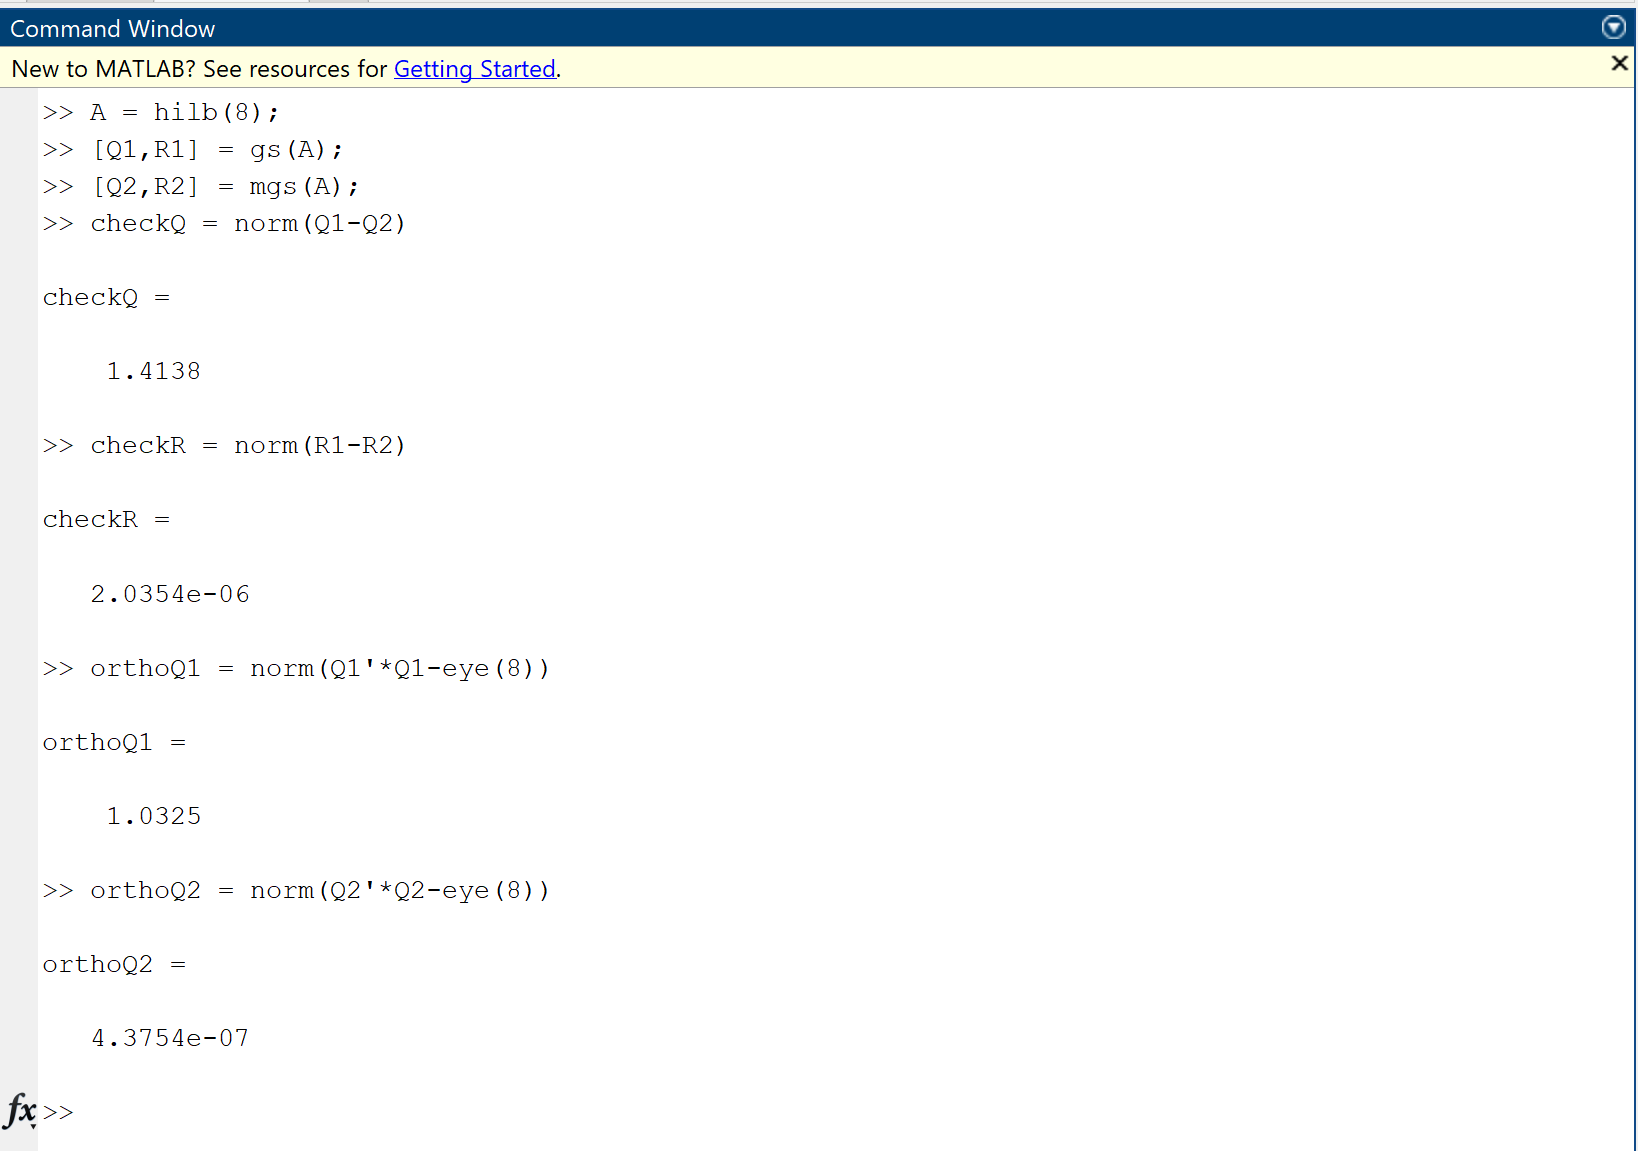
\includegraphics{question5.png}


\end{document}